\chapter{Comparing Decomposition Implementations \TO}\label{Chapter:benchmark-results}
In Section~\ref{Subsection:implementation-decomposition-project-benchmark} the benchmark structure implemented in order to compare the performance of the GPU version of the LU decomposition and the CPU version was presented. During the development of the project the benchmark was run on many different platforms, such as, smaller compute servers, or the HELIOS cluster\footnote{HELIOS cluster documentation URL: \url{http://helios.fjfi.cvut.cz/}} belonging to the Department of Mathematics; both are found in the Faculty of Nuclear Sciences and Physical Engineering of the Czech Technical University in Prague. This chapter will present and analyze the results of the benchmark that was run in order to compare the two aforementioned implementations. To begin with, the benchmarked implementations will be briefly summarized along with the specifications of the platform that the benchmarks were run on. Then, the set of matrices used in the benchmarks will be presented. Finally, the results of the benchmark will be presented and analyzed.

\section{Benchmarked Implementations \TO}\label{Section:benchmark-results-benchmarked-implementations}
The implementations in the \textit{Decomposition} project that were benchmarked are the following:

\begin{itemize}
	\item \textit{\nameref{Paragraph:implementation-decomposition-project-lu-decomposition-crout-method}} (CM) - This implementation is only available for the CPU. At its core, it is a sequential algorithm that delivers a decomposition of the input matrix in one pass.
	\item \textit{\nameref{Paragraph:implementation-decomposition-project-lu-decomposition-iterative-crout-method}} (ICM$ x $) - This implementation is available only for the GPU. At its core, it is an iterative and parallelizable algorithm that converges to an approximate decomposition of the input matrix. This implementation was further divided into three different configurations of threads per block (denoted by $ x $): $ 8\times 8 $ (ICM8), $ 16\times 16 $ (ICM16), and $ 32\times 32 $ (ICM32); ICM$ x $ refers to all three configurations.
\end{itemize}



\section{Benchmark Platform Specifications \TO}\label{Section:benchmark-results-benchmark-platform-specifications}
The benchmark was run on the RCI (Research Center for Informatics in CTU Prague) Cluster\footnote{RCI homepage URL: \url{http://rci.cvut.cz/}} which is a HPC (High Performance Computing) infrastructure intended for use mainly by researchers. It is made up of CPU, GPU, and SMP nodes that are interconnected by a 100Gbit low-latency network \cite{VVJW5lCpZRWyg8xc}. The hardware and software specifications of the cluster node that the benchmarks were run on can be found in Table~\ref{Table:benchmark-results-benchmark-platform-specifications}.

\begin{table}[h!]
	\centering
	\begin{tabular}{|l|l|}
		\hline
		CPU              & AMD EPYC 7543@3.1GHz (32 cores, 64 threads) \\
		RAM              & 32GB RAM \\
		GPU              & Nvidia Tesla A100 40GB HBM2 (1.6 TByte/s memory bandwidth) \\
		Operating System & CentOS 8 Linux \\
		Compiler         & GCC 10.3 \\
		CUDA             & CUDA 11.4.1 \\ \hline
	\end{tabular}
	\caption{Specifications of the \code{gpu} RCI Cluster node that the benchmarks were run on. Taken from \emph{RCI Cluster Hardware} \cite{VVJW5lCpZRWyg8xc} and the configuration of the computation job.}
	\label{Table:benchmark-results-benchmark-platform-specifications}
\end{table}



\section{Matrices Used for Benchmarks \TO}
The benchmarks for the implementations were run on a set of $ 63 $ matrices. The number of matrices used is comparatively smaller compared to the set of matrices used in the benchmarks of the author's bachelor thesis \textit{Formats for storage of sparse matrices on GPU} \cite{Cejka2020}. The lack of matrices in this benchmark is due to the fact that the current version of the \textit{Decomposition} project does not support decomposition of matrices that are not strongly regular, i.e. matrices that require a permutation matrix for a successful decomposition - described in Section~\ref{Section:theory-lu-decomposition}. This means that any matrices used in the benchmark had to be checked for the aforementioned requirement which made the selection process lengthy. Furthermore, since some dense matrices were included in the set, the drive space required was nearing the limit of what was feasible to move between servers and store in a compute node's scratch memory.
\par The majority of matrices from the set used are sparse as they were obtained from the \emph{SuiteSparse Matrix Collection} \cite{Davis2011}. The remaining matrices are dense - they were randomly generated using the Python script shown in Listing~\ref{Listing:random-dense-matrix-generator} in Attachment~\ref{Attachment:random-dense-matrix-generator}. The dimensions of the matrices in the set ranged from $ 27 \times 27 $ to $ 10,793 \times 10,793 $ and, in general, their nonzero elements were mostly located along the main diagonal with some exceptions. For the direct comparison of results $ 14 $ matrices were selected from the set of $ 63 $. The chosen matrices were selected to represent a wide variety of characteristics: density/sparsity, nonzero element structure, and dimensions. The $ 14 $ selected matrices can be found in Table~\ref{Table:benchmark-results-matrices-used-for-benchmarks-14-selected-matrices}.

\begin{table}[h!]
	\centering
	\begin{tabular}{|>{\footnotesize}l|>{\raggedleft\arraybackslash\footnotesize}r|>{\raggedleft\arraybackslash\footnotesize}r|>{\raggedleft\arraybackslash\footnotesize}r|>{\raggedleft\arraybackslash\footnotesize}r|}
		\hline
		\multicolumn{1}{|>{\centering\footnotesize}c|}{Matrix} & \multicolumn{1}{>{\centering\footnotesize}c|}{Rows} & \multicolumn{1}{>{\centering\footnotesize}c|}{Columns} & \multicolumn{1}{>{\centering\footnotesize}c|}{Nonzeros} & \multicolumn{1}{>{\centering\footnotesize}c|}{Avg. nonzeros per row} \\ \hline
		bcsstk03        &    112 &    112 &         640 &      5.7 \\
		494\_bus 		&    494 &    494 &       1,666 &      3.4 \\
		LeGresley\_2508 &  2,508 &  2,508 &      16,727 &      6.7 \\
		Cejka2842		&  2,842 &  2,842 &   8,076,964 &  2,842.0 \\
		rail\_5177      &  5,177 &  5,177 &      35,185 &      6.8 \\
		c-31		    &  5,339 &  5,339 &      78,571 &     14.7 \\
		s3rmt3m3        &  5,357 &  5,357 &     207,123 &     38.7 \\
		s1rmq4m1        &  5,489 &  5,489 &     262,411 &     47.8 \\
		Na5             &  5,832 &  5,832 &     305,630 &  	  52.4 \\
		Cejka5943		&  5,943 &  5,943 &  35,319,249 &  5,943.0 \\
		fp              &  7,548 &  7,548 &     834,222 &    110.5 \\
		Cejka7580		&  7,580 &  7,580 &  57,456,400 &  7,580.0 \\
		bundle1         & 10,581 & 10,581 &  	770,811 &     72.8 \\
		Cejka10793      & 10,793 & 10,793 & 116,488,849 & 10,793.0 \\ \hline
	\end{tabular}
	\caption{Set of $ 14 $ selected matrices from the \emph{The university of Florida sparse matrix collection} \cite{Davis2011} and randomly generated dense matrices (labeled \textit{Cejka<num\_rows>}) that was used for the direct comparison of implementations.}
	\label{Table:benchmark-results-matrices-used-for-benchmarks-14-selected-matrices}
\end{table}



\section{Benchmark Results \TO}
This section will present and analyze the benchmark results obtained from decomposing the matrices shown in Table~\ref{Table:benchmark-results-matrices-used-for-benchmarks-14-selected-matrices} using the implementations mentioned in Section~\ref{Section:benchmark-results-benchmarked-implementations} on the platform described in Section~\ref{Section:benchmark-results-benchmark-platform-specifications}. The benchmark subroutine described in Section~\ref{Subsection:implementation-decomposition-project-benchmark} assumed that each matrix is decomposed once, however, in this benchmark run, in order to minimize anomalous behaviors and assure the quality of presented results, each matrix was decomposed $ 100 $ times. Then, the data collected across all $ 100 $ runs (execution time, bandwidth, speedup, etc.) was averaged and subsequently logged. First, the terminology that will be used during the analysis will be introduced for clarity. Then, benchmark results for both single and double precision comparing the bandwidths achieved by CM and different ICM$ x $ implementations will be presented. Following that, the comparison of speedup between CM and ICM$ x $ will be detailed for both single and double precision. Last but not least, benchmark results across the entire set of $ 63 $ matrices will be briefly shown, along with the accuracy of results for all matrices. Finally, the benchmark results measured during development for the optimizations described in Section~\ref{Section:implementation-optimization} will be shown. Full benchmarks results - including logs - are available upon request, or they can be found in the CD attached.

\paragraph{Benchmark Terminology} The terminology used in the analysis of the benchmark results is both common and adjusted to this project. It will be briefly explained in the context of the benchmark below:

\begin{itemize}
	\item \textbf{Bandwidth} - The amount of data that can be read from or written to device memory by the device within a specified time interval \cite{F4RUu4doMdeEMKXX}. This rate of data transfer is measured in Bytes per second (Byte/s), however, given the evolution in computation it is most-often measured in Gigabytes (GByte/s) - or even Terabytes (TByte/s) with the recently launched Nvidia A100 as shown in Table~\ref{Table:Nvidia-gpu-details-comparison}. According to Section~8.2.2 in \emph{CUDA C++ Best Practices Guide} \cite{F4RUu4doMdeEMKXX} effective bandwidth is defined as
		\begin{equation}
			\frac{\left(B_r + B_w\right)/10^9}{execution\_time} \nonumber\,,
		\end{equation}
	where $ B_r $ refers to the number of bytes read per kernel, $ B_w $ is the number of bytes written per kernel, and the unit of measurement for $ execution\_time $ is seconds. Since the implementations all read from three instances of \code{DenseMatrix} and the write to two during computation (not counting loops), then the numerator can be generalized as:
		\begin{equation}
			\frac{mtx\_rows \cdot mtx\_cols \cdot 5 \cdot \mathrm{sizeof} \left(Real\right)}{10^9} \nonumber\,.
		\end{equation}
	Where $ mtx\_rows $ represents the number of rows of the input matrix; $ mtx\_cols $ represents the number of columns of the input matrix; $ Real $ denotes the precision, which is either single (\code{float}) or double (\code{double}). The '$ 5 $' signifies the reading from three matrices (\code{A}, \code{Z}, and \code{Znew}) and writing to two matrices (\code{Z} and \code{Znew}).
	\item \textbf{Time} - The execution time of the \code{CroutMethodIterative::decompose()} method. In other words, not only the kernel, but also the setup of the computation and copying the required data from the host to device was incorporated into execution time.
\end{itemize}

\subsection{Bandwidth of the Implementations \TO}\label{Subsection:benchmark-results-bandwidth-of-the-implementations}
The bandwidth of the decomposition implementations on the set of matrices using single and double precision is shown in Figure~\ref{Graph:benchmark-results-bandwidth-of-the-implementations-single-double-precision} - note that the graphs in the figure have a $ \log $-scaled vertical axis for clearer presentation of differences between the individual implementations.

\begin{figure}[h!]
	\centering
	\tikzset{mark options={mark size=2.0, line width=0.5pt},font=\small}
	\begin{subfigure}{\textwidth}
		\begin{tikzpicture}
			\begin{axis}
				[
				,width=0.8\textwidth
				,height=0.45\textwidth
				,axis x line*=bottom
				,axis y line*=left
				,xlabel=\textbf{Matrix}
				,x label style={at={(axis description cs:0.575,-0.35)}}
				,ylabel=\textbf{GByte/s} ($ \log $ scale)
				,xmin=-.5, xmax=13.5
				,ymode=log
				,xtick=data,
				,xticklabels={bcsstk03,494\_bus,LeGresley\_2508,Cejka2842,rail\_5177,c-31,s3rmt3m3,s1rmq4m1,Na5,Cejka5943,fp,Cejka7580,bundle1,Cejka10793}
				,x tick label style={rotate=45,anchor=east,yshift=-6pt,align=right}
				,ymajorgrids
				,legend pos=outer north east
				]
				\addplot[black,mark=triangle*] table [x=id, y=cm-bandwidth, col sep=comma] {resources/plot-csv-files/14-matrices-single-precision-rci.csv};
				\addplot[red,mark=x] table [x=id, y=icm8-bandwidth, col sep=comma] {resources/plot-csv-files/14-matrices-single-precision-rci.csv};
				\addplot[green!60!black,mark=square*] table [x=id, y=icm16-bandwidth, col sep=comma] {resources/plot-csv-files/14-matrices-single-precision-rci.csv};
				\addplot[blue,mark=triangle*] table [x=id, y=icm32-bandwidth, col sep=comma] {resources/plot-csv-files/14-matrices-single-precision-rci.csv};
				\legend{CM, ICM8, ICM16, ICM32}
			\end{axis}
		\end{tikzpicture}
		\subcaption{Single precision}
	\end{subfigure}
	\begin{subfigure}{\textwidth}
		\begin{tikzpicture}
			\begin{axis}
				[
				,width=0.8\textwidth
				,height=0.45\textwidth
				,axis x line*=bottom
				,axis y line*=left
				,xlabel=\textbf{Matrix}
				,x label style={at={(axis description cs:0.575,-0.35)}}
				,ylabel=\textbf{GByte/s} ($ \log $ scale)
				,xmin=-.5, xmax=13.5
				,ymode=log
				,xtick=data,
				,xticklabels={bcsstk03,494\_bus,LeGresley\_2508,Cejka2842,rail\_5177,c-31,s3rmt3m3,s1rmq4m1,Na5,Cejka5943,fp,Cejka7580,bundle1,Cejka10793}
				,x tick label style={rotate=45,anchor=east,yshift=-6pt,align=right}
				,ymajorgrids
				,legend pos=outer north east
				]
				\addplot[black,mark=triangle*] table [x=id, y=cm-bandwidth, col sep=comma] {resources/plot-csv-files/14-matrices-double-precision-rci.csv};
				\addplot[red,mark=x] table [x=id, y=icm8-bandwidth, col sep=comma] {resources/plot-csv-files/14-matrices-double-precision-rci.csv};
				\addplot[green!60!black,mark=square*] table [x=id, y=icm16-bandwidth, col sep=comma] {resources/plot-csv-files/14-matrices-double-precision-rci.csv};
				\addplot[blue,mark=triangle*] table [x=id, y=icm32-bandwidth, col sep=comma] {resources/plot-csv-files/14-matrices-double-precision-rci.csv};
				\legend{CM, ICM8, ICM16, ICM32}
			\end{axis}
		\end{tikzpicture}
		\subcaption{Double precision}
	\end{subfigure}
	\caption{Bandwidth achieved by the decomposition implementations on the set of matrices (Table~\ref{Table:benchmark-results-matrices-used-for-benchmarks-14-selected-matrices}) using single and double precision. The vertical axis is $ \log $-scaled for better visibility of differences between implementations.}
	\label{Graph:benchmark-results-bandwidth-of-the-implementations-single-double-precision}
\end{figure}

Overall, no implementation outperformed the rest on all matrices. However, there seems to be a trend in ICM16 and ICM32 achieving a higher bandwidth on average for both single and double precision. The highest bandwidths achieved for single precision were 12.01 GByte/s by ICM16 and 11.92 GByte/s by ICM32 on the \textit{s1rmq4m1} matrix, and 10.70 GByte/s by ICM16 on the \textit{Na5} matrix. In terms of double precision the highest bandwidths achieved were 16.87 GByte/s by ICM32, 14.29 GByte/s by ICM16, and 11.38 GByte/s by ICM8 - all on the \textit{s1rmq4m1} matrix. Matrices \textit{s1rmq4m1} and \textit{Na5} are shown in Figure~\ref{Figure:benchmark-results-bandwidth-of-the-implementations-matrices-s1rmq4m1-na5}.

\begin{figure}[h!]
	\centering
	\begin{subfigure}{.5\textwidth}
		\centering
		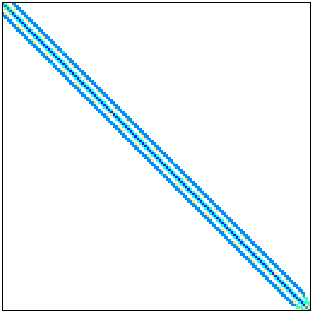
\includegraphics[width=.7\textwidth, keepaspectratio, clip]{Images/ch3/matrices/s1rmq4m1.png}
		\subcaption{s1rmq4m1}
		\label{Subfigure:benchmark-results-bandwidth-of-the-implementations-matrix-s1rmq4m1}
	\end{subfigure}%
	\begin{subfigure}{.5\textwidth}
		\centering
		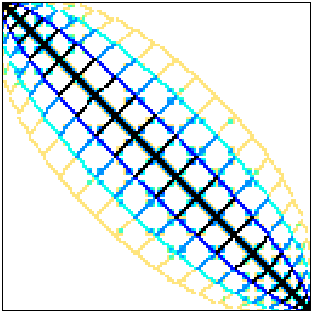
\includegraphics[width=.7\textwidth, keepaspectratio, clip]{Images/ch3/matrices/na5.png}
		\subcaption{Na5}
		\label{Subfigure:benchmark-results-bandwidth-of-the-implementations-matrix-na5}
	\end{subfigure}
	\caption{Nonzero element pattern of the \textit{s1rmq4m1} and \textit{Na5} matrices. Taken from the \emph{The university of Florida sparse matrix collection} \cite{Davis2011}.}
	\label{Figure:benchmark-results-bandwidth-of-the-implementations-matrices-s1rmq4m1-na5}
\end{figure}

As can be seen from Figure~\ref{Subfigure:benchmark-results-bandwidth-of-the-implementations-matrix-s1rmq4m1}, matrix \textit{s1rmq4m1} has nonzero elements on and near its main diagonal. Thus, the matrices arising from the decomposition ($ \mathbb{L} $ and $ \mathbb{U} $, or $ \mathbb{Z} $) will also have elements mainly around their main diagonals. From the perspective of ICM$ x $ this means that the majority of elements requiring computation are found within diagonal sections, therefore, more iterations are required to converge them. On the other hand, non-diagonal sections do not require as many iterations to converge as they contain mostly zeros. Consequently, ICM$ x $ is able to leverage the fact that each diagonal section has the device's resources available to itself and that non-diagonal sections converge in fewer iterations which results in a fast decomposition of the input matrix. In other words, ICM$ x $ is efficient at decomposing n-diagonal sparse matrices, i.e. matrices that have a small number (n) of nonzero diagonals near the main nonzero diagonal. For the \textit{s1rmq4m1} matrix - using either precision - the optimal number of threads per block is either $ 16 \times 16 $ or $ 32 \times 32 $. \\
Similarly, the \textit{Na5} matrix (Figure~\ref{Subfigure:benchmark-results-bandwidth-of-the-implementations-matrix-na5}) has more so an n-diagonal nonzero element structure with minor protrusions in the center. However, the protrusions do not impact the performance severely since the concentration of nonzero elements on the main diagonal is greater than that of the outer diagonals. Therefore, ICM$ x $ also benefits from the fact that, overall, fewer iterations are required to converge to an approximate solution.
\par Conversely, ICM$ x $ achieved its lowest bandwidth across all dense matrices when using double precision. Since the dense matrices used contain only nonzero elements, every section needed many iterations to be converged which in turn meant that, overall, more iterations were needed to converge the entire matrix. For context, the \textit{Cejka5943} dense matrix was decomposed by ICM32 in $ 44.53 $ seconds (using double precision), whereas the \textit{Na5} matrix was decomposed in $ 0.12 $ seconds. On the other hand, when single precision was used, the noticeable difference in performance between sparse and dense matrices was not as prominent. While the reason behind the stark performance difference between single and double precision for ICM$ x $ on dense matrices remains unproven, high-speed shared memory access and generally faster operations using single precision are suspected to be the root causes.
\par ICM$ x $ achieved higher bandwidths on all sparse matrix with the exception of the \textit{bcsstk03} (Figure~\ref{Subfigure:benchmark-results-bandwidth-of-the-implementations-matrix-bcsstk03}) and \textit{rail\_5177} (Figure~\ref{Subfigure:benchmark-results-bandwidth-of-the-implementations-matrix-rail_5177}) matrices despite the former's nonzero element structure being favorable to ICM$ x $. As Table~\ref{Table:benchmark-results-matrices-used-for-benchmarks-14-selected-matrices} lists, the dimensions of the \textit{bcsstk03} matrix are $ 112\times 112 $ which is advantageous for the sequential implementation of CM, as there are fewer steps to perform. Furthermore, since the matrix was already present in host memory, CM's decomposition procedure began without delay. On the other hand, for ICM$ x $, the matrix first had to be copied to device memory and, additionally, the pre-kernel overhead subroutine of ICM$ x $ took - in this case - relatively valuable time to complete. This, combined with the fact that the strength of the iterative algorithm lies in the GPU's ability to process larger datasets, indicates that CM is more suitable for decomposing smaller matrices. \\
When it comes to the \textit{rail\_5177} matrix (Figure~\ref{Subfigure:benchmark-results-bandwidth-of-the-implementations-matrix-rail_5177}), irrespective of the fact that its main diagonal is heavily populated with nonzero elements, there are other nonzero elements interspersed in a seemingly random fashion throughout the matrix. Therefore, similarly to dense matrices, the non-diagonal sections of this matrix also require more iterations to converge.

\begin{figure}[h!]
	\centering
	\begin{subfigure}{.5\textwidth}
		\centering
		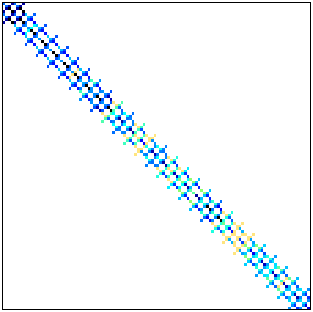
\includegraphics[width=.7\textwidth, keepaspectratio, clip]{Images/ch3/matrices/bcsstk03.png}
		\subcaption{bcsstk03}
		\label{Subfigure:benchmark-results-bandwidth-of-the-implementations-matrix-bcsstk03}
	\end{subfigure}%
	\begin{subfigure}{.5\textwidth}
		\centering
		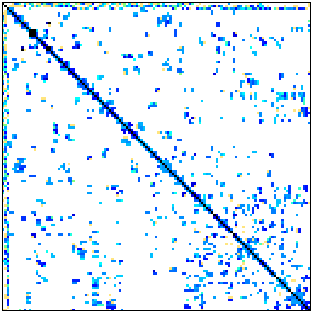
\includegraphics[width=.7\textwidth, keepaspectratio, clip]{images/ch3/matrices/rail_5177.png}
		\subcaption{rail\_5177}
		\label{Subfigure:benchmark-results-bandwidth-of-the-implementations-matrix-rail_5177}
	\end{subfigure}
	\caption{Nonzero element pattern of the \textit{bcsstk03} and \textit{rail\_5177} matrices. Taken from the \emph{The university of Florida sparse matrix collection} \cite{Davis2011}.}
	\label{Figure:benchmark-results-bandwidth-of-the-implementations-matrices-rail_5177-bcsstk03}
\end{figure}

The performance of ICM8 - as shown in Figure~\ref{Graph:benchmark-results-bandwidth-of-the-implementations-single-double-precision} - brings some interesting results. In general, its performance follows that of ICM16 and ICM32, however, some anomalous behavior is present in both single and double precision. For the former, bandwidths achieved seem to be slightly lower for the first $ 10 $ matrices (\textit{bcsstk03} to \textit{Cejka5943}), however, they are considerably lower the larger the matrix dimensions become. This behavior is most likely a result of global memory access becoming a greater bottleneck for single precision when decomposing larger matrices. Consequently, as non-coalesced global memory access is more common for ICM8 than for ICM16, or ICM32 (detailed further in Section~\ref{Subsection:benchmark-results-speedup-comparison-between-CM-and-different-ICMs}), its performance is proportionately lower. For double precision, ICM8 retains the relative performance difference compared to single precision. This is true even when it comes to the \textit{LeGresley\_2508} matrix (Figure~\ref{Figure:benchmark-results-bandwidth-of-the-implementations-matrix-legresley_2508}) which cannot be said about ICM16 and ICM32.

\begin{wrapfigure}{r}{.5\textwidth}
	\centering
	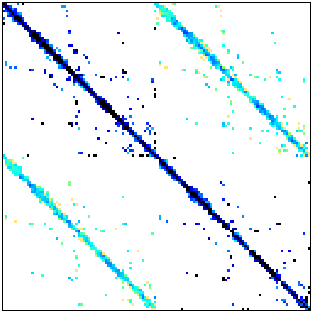
\includegraphics[width=.35\textwidth, keepaspectratio, clip]{images/ch3/matrices/legresley_2508.png}
	\caption{Nonzero element pattern of the \mbox{\textit{LeGresley\_2508}} matrix. Taken from the \emph{The university of Florida sparse matrix collection} \cite{Davis2011}.}
	\label{Figure:benchmark-results-bandwidth-of-the-implementations-matrix-legresley_2508}
\end{wrapfigure}

When comparing the differences in performance over all matrices between single and double precision for ICM16 and ICM32, the results seem consistent with the exception of certain dense matrices and the \textit{LeGresley\_2508} matrix (Figure~\ref{Figure:benchmark-results-bandwidth-of-the-implementations-matrix-legresley_2508}). When double precision is used, the performance of the mentioned implementations decreased drastically compared to single precision and compared to the decrease in performance of ICM8. Since $ 1/10 $ of the matrix dimensions are $ 250.8 $, \code{sectionSize} is set to \code{256} - the edge of the interval. Thus, \code{sectionSize} is the same for ICM8, ICM16, and ICM32 as their respective \code{BLOCK\_SIZE} is a divisor of \code{256}. Therefore, from the perspective of software, the only difference between the implementations in this instance - except for the precision - is the different \code{BLOCK\_SIZE}. It can be argued that ICM8 performed better due to the greater granularity of its thread blocks combined with the smaller size of the matrix. The greater granularity stems from the fact that ICM8 had $ 32 $ blocks assigned to each SM, whereas ICM16 had $ 8 $ and ICM32 had $ 2 $ - the A100 has a maximum of 2048 threads (64 warps; 32 blocks) per SM \cite{soj8qSRbfefUdi8Y}. This means that if the GPU would run out of resources in terms of concurrently active threads, then ICM8 would fair better as its smaller blocks could fill up the remaining resources more tightly (detailed in \textit{\nameref{Paragraph:CUDA-thread-management-grid}} in Section~\ref{Paragraph:CUDA-thread-management-grid}). This effect is only observed when decomposing smaller matrices which have a nonzero element structure similar to that of \textit{LeGresley\_2508}, i.e. matrices with nonzero elements on the main diagonal and nonzero elements interspersed elsewhere. Figure~\ref{Graph:benchmark-results-performance-of-implementations-across-all-matrices-bandwidth-double-precision} further confirms this suspicion for certain matrices where ICM8 outperforms ICM16 and ICM32 when double precision is used. For matrices with larger dimensions this effect would be mitigated since being able to utilize a few additional blocks would not amount to such a drastic difference in performance. Furthermore, the non-coalesced global memory access present for ICM8 (more so than ICM16) becomes apparent when decomposing larger matrices - especially when using single precision.
\par Other than the notable bandwidth achieved on the \textit{bcsstk03} matrix, in general, the performance of CM was lower than that of ICM$ x $ - especially when single precision was used. Conversely, when double precision was used, its performance on dense matrices was comparable to that of ICM$ x $. Specifically, the bandwidth achieved for matrices \textit{Cejka2842}, \textit{Cejka5943}, \textit{Cejka7580}, and \textit{Cejka10793} by CM and ICM32 (best ICM$ x $ for the matrices mentioned) can be seen in Table~\ref{Table:benchmark-results-bandwidth-of-the-implementations-dense-matrices-bandwidth}.

\begin{table}[h!]
	\centering
	\renewcommand{\arraystretch}{1.5}
	\begin{tabular}{ |c|c|c|c|c| } 
		\hline
		Implementation & Cejka2842 & Cejka5943 & Cejka7580 & Cejka10793 \\
		\hline
		CM             &     0.047 &     0.014 &     0.014 & 0.007      \\
		\hline
		ICM32          &     0.093 &     0.032 &     0.021 & 0.011      \\
		\hline
	\end{tabular}
	\caption{Bandwidth achieved (in GByte/s) when decomposing the subset of dense matrices from Table~\ref{Table:benchmark-results-matrices-used-for-benchmarks-14-selected-matrices} by CM and ICM32 using double precision.}
	\label{Table:benchmark-results-bandwidth-of-the-implementations-dense-matrices-bandwidth}
\end{table}

Since the algorithm used for CM is sequential and computes every element of the resulting decomposed matrix $ \mathbb{Z} $ regardless of its value, then there is no difference in how it computes matrices with distinct nonzero element structures. However, it can be argued that - especially when double precision is used - sparse matrices are, in general, decomposed slightly faster than dense matrices with the same dimensions. This is due to the fact that the multiplication and addition operations performed will be working with zeros in the majority of cases. Nevertheless, it can be concluded that the performance of CM is determined more so by the dimensions of a matrix, rather than its nonzero element structure.


\subsection{Speedup Comparison Between CM and different ICMs \TO}\label{Subsection:benchmark-results-speedup-comparison-between-CM-and-different-ICMs}
As the bandwidth results shown in Figure~\ref{Graph:benchmark-results-bandwidth-of-the-implementations-single-double-precision} are presented with a $ \log $-scaled vertical axis, it can be difficult to see the performance differences between implementations. Therefore, to put the results into perspective, this section presents the speedup comparison between the implementations listed in Section~\ref{Section:benchmark-results-benchmarked-implementations}. Specifically, as mentioned in \textit{\nameref{Paragraph:implementation-decomposition-project-lu-decomposition-implementation-requirements}} in Section~\ref{Paragraph:implementation-decomposition-project-lu-decomposition-implementation-requirements} one of the goals of this project was to "\textit{measure the acceleration of the GPU version of the LU decomposition against the CPU version}". For that reason, speedup from the CM (host) implementation to the ICM$ x $ (device) implementations will be compared. The comparison - using single and double precision - on the set of matrices listed in Table~\ref{Table:benchmark-results-matrices-used-for-benchmarks-14-selected-matrices} is shown in Figure~\ref{Graph:benchmark-results-speedup-comparison-between-CM-and-different-ICMs-single-double-precision}.

\begin{figure}[h!]
	\centering
	\tikzset{mark options={mark size=2.0, line width=0.5pt},font=\small}
	\begin{subfigure}{\textwidth}
		\begin{tikzpicture}
			\begin{axis}
				[
				,width=0.8\textwidth
				,height=0.45\textwidth
				,axis x line*=bottom
				,axis y line*=left
				,xlabel=\textbf{Matrix}
				,x label style={at={(axis description cs:0.575,-0.35)}}
				,ylabel=\textbf{Speedup}
				,xmin=-.5, xmax=13.5
				,ymin=-200, ymax=2100
				,xtick=data,
				,ytick={1, 500, 1000, 1500, 2000}
				,xticklabels={bcsstk03,494\_bus,LeGresley\_2508,Cejka2842,rail\_5177,c-31,s3rmt3m3,s1rmq4m1,Na5,Cejka5943,fp,Cejka7580,bundle1,Cejka10793}
				,x tick label style={rotate=45,anchor=east,yshift=-6pt,align=right}
				,ymajorgrids
				,legend pos=outer north east
				]
				\addplot[black,mark=triangle*] table [x=id, y=cm-speedup, col sep=comma] {resources/plot-csv-files/14-matrices-single-precision-rci.csv};
				\addplot[red,mark=x] table [x=id, y=icm8-speedup, col sep=comma] {resources/plot-csv-files/14-matrices-single-precision-rci.csv};
				\addplot[green!60!black,mark=square*] table [x=id, y=icm16-speedup, col sep=comma] {resources/plot-csv-files/14-matrices-single-precision-rci.csv};
				\addplot[blue,mark=triangle*] table [x=id, y=icm32-speedup, col sep=comma] {resources/plot-csv-files/14-matrices-single-precision-rci.csv};
				\legend{CM, ICM8, ICM16, ICM32}
			\end{axis}
		\end{tikzpicture}
		\subcaption{Single precision}
		\label{Graph:benchmark-results-speedup-comparison-between-CM-and-different-ICMs-single-precision}
	\end{subfigure}
	\begin{subfigure}{\textwidth}
		\begin{tikzpicture}
			\begin{axis}
				[
				,width=0.8\textwidth
				,height=0.45\textwidth
				,axis x line*=bottom
				,axis y line*=left
				,xlabel=\textbf{Matrix}
				,x label style={at={(axis description cs:0.575,-0.35)}}
				,ylabel=\textbf{Speedup}
				,xmin=-.5, xmax=13.5
				,ymin=-200, ymax=2100
				,ytick={1, 500, 1000, 1500, 2000}
				,xtick=data,
				,xticklabels={bcsstk03,494\_bus,LeGresley\_2508,Cejka2842,rail\_5177,c-31,s3rmt3m3,s1rmq4m1,Na5,Cejka5943,fp,Cejka7580,bundle1,Cejka10793}
				,x tick label style={rotate=45,anchor=east,yshift=-6pt,align=right}
				,ymajorgrids
				,legend pos=outer north east
				]
				\addplot[black,mark=triangle*] table [x=id, y=cm-speedup, col sep=comma] {resources/plot-csv-files/14-matrices-double-precision-rci.csv};
				\addplot[red,mark=x] table [x=id, y=icm8-speedup, col sep=comma] {resources/plot-csv-files/14-matrices-double-precision-rci.csv};
				\addplot[green!60!black,mark=square*] table [x=id, y=icm16-speedup, col sep=comma] {resources/plot-csv-files/14-matrices-double-precision-rci.csv};
				\addplot[blue,mark=triangle*] table [x=id, y=icm32-speedup, col sep=comma] {resources/plot-csv-files/14-matrices-double-precision-rci.csv};
				\legend{CM, ICM8, ICM16, ICM32}
			\end{axis}
		\end{tikzpicture}
		\subcaption{Double precision}
	\end{subfigure}
	\caption{Speedup comparison between the decomposition times of CM and the ICM$ x $ implementations on the set of matrices (Table~\ref{Table:benchmark-results-matrices-used-for-benchmarks-14-selected-matrices}) using single and double precision. }
	\label{Graph:benchmark-results-speedup-comparison-between-CM-and-different-ICMs-single-double-precision}
\end{figure}

\paragraph{ICM16 and ICM32} Similarly to the bandwidth results, overall, ICM16 and ICM32 were the best-performing implementations. For single precision, the three highest speedups compared to CM were $ 2030.30 $ by ICM32 and $ 1803.08 $ by ICM16 on the \textit{bundle1} matrix (Figure~\ref{Subfigure:benchmark-results-speedup-comparison-between-CM-and-different-ICMs-matrix-bundle1}), and $ 1352.55 $ by ICM16 on the \textit{s1rmq4m1} matrix (Figure~\ref{Subfigure:benchmark-results-bandwidth-of-the-implementations-matrix-s1rmq4m1}). In terms of double precision, the highest speedups compared to CM were $ 1337.53 $ and $ 1137.98 $ achieved by ICM32 on matrices \textit{bundle1} and \textit{s1rmq4m1} respectively, and $ 1022.01 $ achieved by ICM16 on the \textit{bundle1} matrix.

\begin{figure}[h!]
	\centering
	\begin{subfigure}{.5\textwidth}
		\centering
		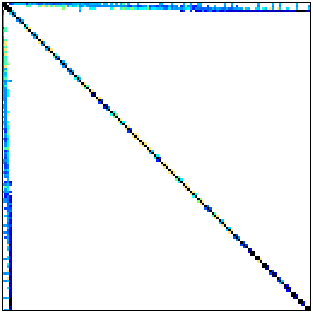
\includegraphics[width=.7\textwidth, keepaspectratio, clip]{Images/ch3/matrices/bundle1.png}
		\subcaption{bundle1}
		\label{Subfigure:benchmark-results-speedup-comparison-between-CM-and-different-ICMs-matrix-bundle1}
	\end{subfigure}%
	\begin{subfigure}{.5\textwidth}
		\centering
		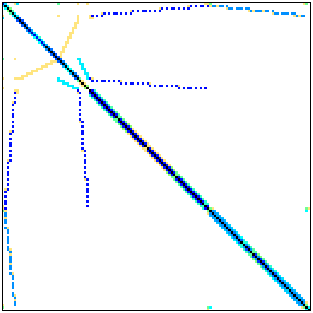
\includegraphics[width=.7\textwidth, keepaspectratio, clip]{images/ch3/matrices/s3rmt3m3.png}
		\subcaption{s3rmt3m3}
		\label{Subfigure:benchmark-results-speedup-comparison-between-CM-and-different-ICMs-matrix-s3rmt3m3}
	\end{subfigure}
	\caption{Nonzero element pattern of the \textit{bundle1} and \textit{s3rmt3m3} matrices. Taken from the \emph{The university of Florida sparse matrix collection} \cite{Davis2011}.}
	\label{Figure:benchmark-results-speedup-comparison-between-CM-and-different-ICMs-matrices-rail_5177-bcsstk03}
\end{figure}

Nevertheless, there are exceptions to the greater performance of ICM32. One such exception is the speedup compared to ICM8 on the \textit{s3rmt3m3} matrix (Figure~\ref{Subfigure:benchmark-results-speedup-comparison-between-CM-and-different-ICMs-matrix-s3rmt3m3}) when single precision is used. For this matrix, ICM32 achieved a speedup of $ 368.14 $, whereas ICM8 achieved $ 427.55 $. As can be seen from Figure~\ref{Subfigure:benchmark-results-speedup-comparison-between-CM-and-different-ICMs-matrix-s3rmt3m3} the nonzero element structure of the \textit{s3rmt3m3} matrix comprises of a strong concentration of nonzero elements along the main diagonal and six nonzero-element lines aimed away from the main diagonal. The reason mentioned for the higher performance on the \textit{Na5} matrix describes that a matrix with a similar nonzero element structure should not require many iterations to decompose for ICM$ x $ as the main diagonal has most of the nonzero elements and only a few other nonzero elements are found outside it. However, since the nonzero elements found outside the main diagonal are located much further from it than that of the \textit{Na5} matrix pictured in Figure~\ref{Subfigure:benchmark-results-bandwidth-of-the-implementations-matrix-na5}, then the non-diagonal sections needed more iterations to converge.
\par Another noteworthy sparse matrix on which ICM$ x $ struggled - relative to the rest - was the \textit{fp} matrix (Figure~\ref{Figure:benchmark-results-speedup-comparison-between-CM-and-different-ICMs-matrix-fp}). It can be seen that the nonzero element structure is similar to that of the \textit{rail\_5177} matrix (Figure~\ref{Subfigure:benchmark-results-bandwidth-of-the-implementations-matrix-rail_5177}). In other words, nonzero elements are concentrated on the main diagonal and other nonzero elements are interspersed throughout the rest of the matrix. Consequently, the lack of performance by ICM$ x $ is due to more iterations required to converge the non-diagonal sections.

\begin{figure}[h!]
	\centering
	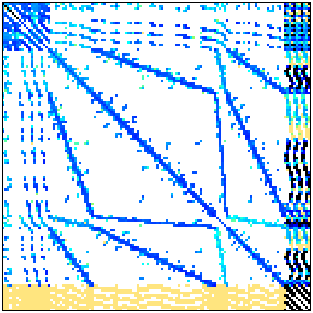
\includegraphics[width=.35\textwidth, keepaspectratio, clip]{images/ch3/matrices/fp.png}
	\caption{Nonzero element pattern of the \mbox{\textit{fp}} matrix. Taken from the \emph{The university of Florida sparse matrix collection} \cite{Davis2011}.}
	\label{Figure:benchmark-results-speedup-comparison-between-CM-and-different-ICMs-matrix-fp}
\end{figure}

\paragraph{ICM8} In general, ICM8 was faster than CM, however, when its speedup is compared to that of ICM16 and ICM32, there is a difference in performance. This difference is noticeable especially for matrices that required few iterations to decompose the entire matrix, for example, \textit{s1rmq4m1}, \textit{Na5}, and \textit{bundle1}. Since the decomposition time for these matrices was - at worst - $ 0.9 $ seconds for each, loading elements from global to shared memory became a bottleneck. The reason behind this stems from the fact that threads in blocks are divided into warps by their \code{threadIdx.x} index. Thus, when reading from shared memory threads in a warp should - ideally - access neighboring global memory addresses. Since elements of the \code{DenseMatrix} instance are stored in row-major order on the GPU, each warp in ICM8 loads elements from global memory in the following way: first 8 threads of the warp read data from neighboring addresses, the next 8 threads of the warp also read from other neighboring addresses, in other words, they are not found near the first 8 addresses (unless the matrix dimensions are $ 8\times 8 $) - this is non-coalesced access to memory. In this instance, the non-coalesced access is the same as depicted in the upper image of Figure~\ref{Sub-figure:CUDA-global-memory-non-coalesced-access-2}. Therefore, as mentioned in the figure's caption, instead of the threads in a warp performing one transaction to global memory, they will perform $ 32/8 = 4 $ sequential transactions (detailed further in \textit{\nameref{Paragraph:CUDA-memory-management-global-memory}} in Section~\ref{Paragraph:CUDA-memory-management-global-memory}). \\
This means that non-coalesced access to global memory occurs for ICM8 and ICM16, however, the latter will only perform $ 32/16 = 2 $ sequential transactions. On the other hand, this defect is not present for ICM32 as the threads of a warp access \code{BLOCK\_SIZE = 32} neighboring addresses in global memory. This effect is apparent in Figure~\ref{Graph:benchmark-results-speedup-comparison-between-CM-and-different-ICMs-single-double-precision} (ICM32 performed better than ICM16 which outperformed ICM8), especially when decomposing the previously-mentioned matrices: \textit{s1rmq4m1}, \textit{Na5} and \textit{bundle1} using double precision.
\paragraph{CM}\label{Paragraph:benchmark-results-speedup-comparison-between-CM-and-different-ICMs-CM-speedup-description}
In Figure~\ref{Graph:benchmark-results-speedup-comparison-between-CM-and-different-ICMs-single-double-precision} it can be seen that CM took more time to decompose most of the benchmarked matrices. However, an interesting result arises when comparing CM and ICM8 for double precision. Specifically, for $ 3 $ out of the $ 14 $ matrices, ICM8 was slower than CM as it achieved the following speedups: $ 0.09 $ for \textit{bcsstk03}, $ 0.92 $ for \textit{Cejka7580}, and $ 0.96 $ for \textit{Cejka10793}. While the result for \textit{bcsstk03} is not surprising given the matrix's dimensions, the others are. The most likely reason for the lower performance is the non-coalesced access to global memory which is most prominent for ICM8.
\par Overall, the decomposition of matrices using single precision was faster compared to double precision. However, the difference in speed is not clearly visible from either Figure~\ref{Graph:benchmark-results-bandwidth-of-the-implementations-single-double-precision} (due to the vertical axis being $ \log $-scaled) or Figure~\ref{Graph:benchmark-results-speedup-comparison-between-CM-and-different-ICMs-single-double-precision} (due to the range of the speedup factor being too great for the values to be distinguishable). For this reason, the raw execution times for single and double precision are included in Table~\ref{Table:benchmark-results-speedup-comparison-between-CM-and-different-ICMs-execution-times-single-precision} and Table~\ref{Table:benchmark-results-speedup-comparison-between-CM-and-different-ICMs-execution-times-double-precision} respectively.

\begin{table}[h!]
	\centering
	\begin{tabular}{|>{\footnotesize}l|>{\raggedleft\arraybackslash\footnotesize}r|>{\raggedleft\arraybackslash\footnotesize}r|>{\raggedleft\arraybackslash\footnotesize}r|>{\raggedleft\arraybackslash\footnotesize}r|}
		\hline
		\multicolumn{1}{|>{\centering\footnotesize}c|}{Matrix} & \multicolumn{1}{>{\centering\footnotesize}c|}{CM} & \multicolumn{1}{>{\centering\footnotesize}c|}{ICM8} & \multicolumn{1}{>{\centering\footnotesize}c|}{ICM16} & \multicolumn{1}{>{\centering\footnotesize}c|}{ICM32} \\ \hline
		bcsstk03        & \cellcolor{green!25}0.0002 &  0.0022 &                     0.0020 &                     0.0022 \\
		494\_bus 		&                     0.0292 &  0.0049 &                     0.0053 & \cellcolor{green!25}0.0043 \\
		LeGresley\_2508 &                     4.2193 &  0.0793 & \cellcolor{green!25}0.0498 &                     0.0531 \\
		Cejka2842		&                     6.2210 &  3.0391 & \cellcolor{green!25}2.1182 &                     2.1412 \\
		rail\_5177      &                    55.1124 &  1.4350 & \cellcolor{green!25}1.0669 &                     1.1022 \\
		c-31		    &                    59.3208 &  0.1598 &                     0.1330 & \cellcolor{green!25}0.1327 \\
		s3rmt3m3        &                    61.9867 &  0.1450 & \cellcolor{green!25}0.1133 &                     0.1684 \\
		s1rmq4m1        &                    67.8509 &  0.0641 & \cellcolor{green!25}0.0502 &                     0.0505 \\
		Na5             &                    62.3995 &  0.0817 & \cellcolor{green!25}0.0636 &                     0.0649 \\
		Cejka5943		&                    90.1114 &  0.7035 &                     0.5230 & \cellcolor{green!25}0.4856 \\
		fp              &                   179.7054 &  0.5278 &                     0.3980 & \cellcolor{green!25}0.3690 \\
		Cejka7580		&                   151.7981 & 12.2164 &                     3.0289 & \cellcolor{green!25}2.2853 \\
		bundle1         &                   617.5120 &  0.4853 &                     0.3425 & \cellcolor{green!25}0.3041 \\
		Cejka10793      &                   643.3462 &  9.2837 &                     2.8510 & \cellcolor{green!25}2.2107 \\ \hline
	\end{tabular}
	\caption{The execution time (in seconds) of decomposition for all implementations on the set of matrices (Table~\ref{Table:benchmark-results-matrices-used-for-benchmarks-14-selected-matrices}) using \textbf{single} precision. The fastest time for each matrix is highlighted in green.}
	\label{Table:benchmark-results-speedup-comparison-between-CM-and-different-ICMs-execution-times-single-precision}
\end{table}

\begin{table}[h!]
	\centering
	\begin{tabular}{|>{\footnotesize}l|>{\raggedleft\arraybackslash\footnotesize}r|>{\raggedleft\arraybackslash\footnotesize}r|>{\raggedleft\arraybackslash\footnotesize}r|>{\raggedleft\arraybackslash\footnotesize}r|}
		\hline
		\multicolumn{1}{|>{\centering\footnotesize}c|}{Matrix} & \multicolumn{1}{>{\centering\footnotesize}c|}{CM} & \multicolumn{1}{>{\centering\footnotesize}c|}{ICM8} & \multicolumn{1}{>{\centering\footnotesize}c|}{ICM16} & \multicolumn{1}{>{\centering\footnotesize}c|}{ICM32} \\ \hline
		bcsstk03        & \cellcolor{green!25}0.0003 &                     0.0027 &                     0.0026 &                       0.0027 \\
		494\_bus 		&                     0.0299 &                     0.0084 & \cellcolor{green!25}0.0070 &                       0.0082 \\
		LeGresley\_2508 &                     4.3542 & \cellcolor{green!25}0.2055 &                     0.4805 &                       0.6118 \\
		Cejka2842		&                     6.9110 &                     4.5995 &                     3.6436 & \cellcolor{green!25}  3.4559 \\
		rail\_5177      &                    67.9030 &                     3.0109 &                     2.3882 & \cellcolor{green!25}  2.1754 \\
		c-31		    &                    72.3863 &                     0.4913 &                     0.4166 & \cellcolor{green!25}  0.3349 \\
		s3rmt3m3        &                    74.0106 &                     0.3704 &                     0.2997 & \cellcolor{green!25}  0.2577 \\
		s1rmq4m1        &                    81.2749 &                     0.1059 &                     0.0843 & \cellcolor{green!25}  0.0714 \\
		Na5             &                    67.2166 &                     0.1543 &                     0.1365 & \cellcolor{green!25}  0.1243 \\
		Cejka5943		&                   104.6150 &                    70.8865 &                    56.2768 & \cellcolor{green!25} 44.5275 \\
		fp              &                   154.8232 &                     0.9641 &                     0.7715 & \cellcolor{green!25}  0.6287 \\
		Cejka7580		&                   159.6421 &                   172.9549 &                   138.9242 & \cellcolor{green!25}107.8041 \\
		bundle1         &                   679.3846 &                     0.8859 &                     0.6648 & \cellcolor{green!25}  0.5079 \\
		Cejka10793      &                   699.9634 &                   731.9412 &                   556.0243 & \cellcolor{green!25}419.1401 \\ \hline
	\end{tabular}
	\caption{The execution time (in seconds) of decomposition for all implementations on the set of matrices (Table~\ref{Table:benchmark-results-matrices-used-for-benchmarks-14-selected-matrices}) using \textbf{double} precision. The fastest time for each matrix is highlighted in green.}
	\label{Table:benchmark-results-speedup-comparison-between-CM-and-different-ICMs-execution-times-double-precision}
\end{table}

From the results presented in Table~\ref{Table:benchmark-results-speedup-comparison-between-CM-and-different-ICMs-execution-times-single-precision} it could be concluded that ICM32 is the most suitable implementation for decomposing matrices using single precision. In terms of double precision the same statement could be made when looking at Table~\ref{Table:benchmark-results-speedup-comparison-between-CM-and-different-ICMs-execution-times-double-precision}. However, since the results presented in the mentioned tables were only a small subset of all results, verification of this claim is required for the entire set of $ 63 $ matrices.

\subsection{Performance of Implementations Across All Matrices \TO}\label{Subsection:benchmark-results-performance-of-implementations-across-all-matrices}
This section shows the bandwidth, speedup comparison, and accuracy of results - using both single and double precision - for the decomposition implementations listed in Section~\ref{Section:benchmark-results-benchmarked-implementations}. The metrics were measured across the entire set of 63 matrices and the benchmarks were run on the platform specified in Table~\ref{Table:benchmark-results-benchmark-platform-specifications}. In order to illustrate how ICM$ x $ compares to CM on matrices that increase in size, the matrices in the graphs were sorted from smallest to largest. The bandwidth results can be found in Figure~\ref{Graph:benchmark-results-performance-of-implementations-across-all-matrices-bandwidth-single-double-precision}, the speedup comparison between CM and ICM$ x $ can be found in Figure~\ref{Graph:benchmark-results-performance-of-implementations-across-all-matrices-speedup-single-double-precision}, and the accuracy of the results can be found in Figure~\ref{Graph:benchmark-results-performance-of-implementations-across-all-matrices-accuracy-single-double-precision}. All figures in this section have a $ \log $-scaled vertical axis as the range of values was too great to present any coherent data.

\paragraph{Bandwidth} As shown in Figure~\ref{Graph:benchmark-results-performance-of-implementations-across-all-matrices-bandwidth-single-double-precision}, in terms of bandwidth, the ICM$ x $ implementations achieved similar results with the exception of ICM8 that is noticeably less performant. The lack of ICM8's performance is more prominent for single precision where the issue with non-coalesced global memory access appears to be making a difference. This is further supported by the fact that after a certain point (matrix $ 46 $) ICM8 appears to be consistently falling behind ICM32 in terms of bandwidth achieved - especially noticeable for the larger dense matrices (the three dips in bandwidth after matrix $ 55 $ in Figure~\ref{Graph:benchmark-results-performance-of-implementations-across-all-matrices-bandwidth-single-precision}).
\par In terms of double precision the performance of ICM$ x $ is more consistent. The general rule of ICM8 performing worse than ICM16 and ICM32 for larger matrices still stands and the performance of ICM16 for matrices past matrix $ 30 $ is - in the majority of cases - less than that of ICM32. The dips in bandwidth of ICM$ x $ for matrices past matrix $ 25 $ are caused by the dense matrices found in the set. For the majority of matrices, the bandwidth achieved during their decomposition was greater than 1 GByte/s for both single and double precision. On the other hand, Figure~\ref{Graph:benchmark-results-performance-of-implementations-across-all-matrices-bandwidth-single-double-precision} shows that the bandwidth achieved by CM decreases in an almost logarithmic fashion with increasing matrix dimensions.
\par Contrary to what the subset of results presented in Section~\ref{Subsection:benchmark-results-bandwidth-of-the-implementations} seemed to suggest, it can be seen from Figure~\ref{Graph:benchmark-results-performance-of-implementations-across-all-matrices-bandwidth-single-precision} (single precision) and Figure~\ref{Graph:benchmark-results-performance-of-implementations-across-all-matrices-bandwidth-double-precision} (double precision) that CM outperformed ICM$ x $ in more cases than just one. Although, it must be mentioned that the matrices on which CM achieved a higher bandwidth than ICM$ x $ did have dimensions between $ 27\times 27 $ and $ 415\times 415 $.

\begin{figure}[h!]
	\centering
	\tikzset{mark options={mark size=1.5},font=\small}
	\begin{subfigure}{\textwidth}
		\begin{tikzpicture}
			\begin{axis}
				[
				,width=\textwidth
				,height=0.45\textwidth
				,axis x line*=bottom
				,axis y line*=left
				,xlabel=\textbf{Matrix ID}
				,ylabel=\textbf{GByte/s} ($ \log $ scale)
				,x label style={at={(axis description cs:0.46,-.1)}}
				,xmin=-1, xmax=63
				,ymode=log
				,ymajorgrids
				,legend style={at={(0.5,1.15)},anchor=north,cells={anchor=east},legend columns=-1}
				]
				\addplot[black,mark=*] table [x=id, y=cm-bandwidth, col sep=comma] {resources/plot-csv-files/63-matrices-single-precision-rci.csv};
				\addplot[red,mark=*] table [x=id, y=icm8-bandwidth, col sep=comma] {resources/plot-csv-files/63-matrices-single-precision-rci.csv};
				\addplot[green!60!black,mark=*] table [x=id, y=icm16-bandwidth, col sep=comma] {resources/plot-csv-files/63-matrices-single-precision-rci.csv};
				\addplot[blue,mark=*] table [x=id, y=icm32-bandwidth, col sep=comma] {resources/plot-csv-files/63-matrices-single-precision-rci.csv};
				\legend{CM, ICM8, ICM16, ICM32}
			\end{axis}
		\end{tikzpicture}
		\subcaption{Single precision}
		\label{Graph:benchmark-results-performance-of-implementations-across-all-matrices-bandwidth-single-precision}
	\end{subfigure}
	\vspace{0.25cm}
	\begin{subfigure}{\textwidth}
		\begin{tikzpicture}
			\begin{axis}
				[
				,width=\textwidth
				,height=0.45\textwidth
				,axis x line*=bottom
				,axis y line*=left
				,xlabel=\textbf{Matrix ID}
				,ylabel=\textbf{GByte/s} ($ \log $ scale)
				,x label style={at={(axis description cs:0.46,-.1)}}
				,xmin=-1, xmax=63
				,ymode=log
				,ymajorgrids
				,legend style={at={(0.5,1.15)},anchor=north,cells={anchor=east},legend columns=-1}
				]
				\addplot[black,mark=*] table [x=id, y=cm-bandwidth, col sep=comma] {resources/plot-csv-files/63-matrices-double-precision-rci.csv};
				\addplot[red,mark=*] table [x=id, y=icm8-bandwidth, col sep=comma] {resources/plot-csv-files/63-matrices-double-precision-rci.csv};
				\addplot[green!60!black,mark=*] table [x=id, y=icm16-bandwidth, col sep=comma] {resources/plot-csv-files/63-matrices-double-precision-rci.csv};
				\addplot[blue,mark=*] table [x=id, y=icm32-bandwidth, col sep=comma] {resources/plot-csv-files/63-matrices-double-precision-rci.csv};
				\legend{CM, ICM8, ICM16, ICM32}
			\end{axis}
		\end{tikzpicture}
		\subcaption{Double precision}
		\label{Graph:benchmark-results-performance-of-implementations-across-all-matrices-bandwidth-double-precision}
	\end{subfigure}
	\caption{Bandwidths achieved by decomposition implementations listed in Section~\ref{Section:benchmark-results-benchmarked-implementations} on the entire set of $ 63 $ matrices using both single and double precision. Matrix ID signifies the ID of the matrices, after they have been sorted according to their dimension from smallest to largest. The vertical axis is $ \log $-scaled for better visibility of differences between implementations.}
	\label{Graph:benchmark-results-performance-of-implementations-across-all-matrices-bandwidth-single-double-precision}
\end{figure}

\paragraph{Speedup} The speedup comparison in Figure~\ref{Graph:benchmark-results-performance-of-implementations-across-all-matrices-speedup-single-double-precision} is presented for the sake of completeness and to show how much faster the ICM$ x $ implementations were compared to CM. Specifically, when single precision was used, all ICM$ x $ implementations were faster in $ 54/63 $ cases. In terms of double precision, ICM8 was faster in $ 51/63 $ cases, and ICM32 and ICM16 were faster in $ 53/63 $. However, as mentioned before, all of the matrices (with the two exceptions for ICM8 detailed in \textit{\nameref{Paragraph:benchmark-results-speedup-comparison-between-CM-and-different-ICMs-CM-speedup-description}} in Section~\ref{Paragraph:benchmark-results-speedup-comparison-between-CM-and-different-ICMs-CM-speedup-description}) that CM decomposed faster than ICM$ x $ have dimensions $ 415\times 415 $ or smaller.

\begin{figure}[h!]
	\centering
	\tikzset{mark options={mark size=1.5},font=\small}
	\begin{subfigure}{\textwidth}
		\begin{tikzpicture}
			\begin{axis}
				[
				,width=\textwidth
				,height=0.45\textwidth
				,axis x line*=bottom
				,axis y line*=left
				,xlabel=\textbf{Matrix ID}
				,ylabel=\textbf{Speedup} ($ \log $ scale)
				,x label style={at={(axis description cs:0.46,-.1)}}
				,xmin=-1, xmax=63
				,ymode=log
				,ymajorgrids
				,legend style={at={(0.5,1.15)},anchor=north,cells={anchor=east},legend columns=-1}
				]
				\addplot[black,mark=*] table [x=id, y=cm-speedup, col sep=comma] {resources/plot-csv-files/63-matrices-single-precision-rci.csv};
				\addplot[red,mark=*] table [x=id, y=icm8-speedup, col sep=comma] {resources/plot-csv-files/63-matrices-single-precision-rci.csv};
				\addplot[green!60!black,mark=*] table [x=id, y=icm16-speedup, col sep=comma] {resources/plot-csv-files/63-matrices-single-precision-rci.csv};
				\addplot[blue,mark=*] table [x=id, y=icm32-speedup, col sep=comma] {resources/plot-csv-files/63-matrices-single-precision-rci.csv};
				\legend{CM, ICM8, ICM16, ICM32}
			\end{axis}
		\end{tikzpicture}
		\subcaption{Single precision}
		\label{Graph:benchmark-results-performance-of-implementations-across-all-matrices-speedup-single-precision}
	\end{subfigure}
	\vspace{0.25cm}
	\begin{subfigure}{\textwidth}
		\begin{tikzpicture}
			\begin{axis}
				[
				,width=\textwidth
				,height=0.45\textwidth
				,axis x line*=bottom
				,axis y line*=left
				,xlabel=\textbf{Matrix ID}
				,ylabel=\textbf{Speedup} ($ \log $ scale)
				,x label style={at={(axis description cs:0.46,-.1)}}
				,xmin=-1, xmax=63
				,ymode=log
				,ymajorgrids
				,legend style={at={(0.5,1.15)},anchor=north,cells={anchor=east},legend columns=-1}
				]
				\addplot[black,mark=*] table [x=id, y=cm-speedup, col sep=comma] {resources/plot-csv-files/63-matrices-double-precision-rci.csv};
				\addplot[red,mark=*] table [x=id, y=icm8-speedup, col sep=comma] {resources/plot-csv-files/63-matrices-double-precision-rci.csv};
				\addplot[green!60!black,mark=*] table [x=id, y=icm16-speedup, col sep=comma] {resources/plot-csv-files/63-matrices-double-precision-rci.csv};
				\addplot[blue,mark=*] table [x=id, y=icm32-speedup, col sep=comma] {resources/plot-csv-files/63-matrices-double-precision-rci.csv};
				\legend{CM, ICM8, ICM16, ICM32}
			\end{axis}
		\end{tikzpicture}
		\subcaption{Double precision}
		\label{Graph:benchmark-results-performance-of-implementations-across-all-matrices-speedup-double-precision}
	\end{subfigure}
	\caption{Speedup comparison between CM and ICM$ x $ implementations on the entire set of $ 63 $ matrices using both single and double precision. Matrix ID signifies the ID of the matrices, after they have been sorted according to their dimension from smallest to largest. The vertical axis is $ \log $-scaled for better visibility of differences between implementations.}
	\label{Graph:benchmark-results-performance-of-implementations-across-all-matrices-speedup-single-double-precision}
\end{figure}

Additionally, Table~\ref{Table:benchmark-results-performance-of-implementations-across-all-matrices-total-execution-time-single-double-precision} shows the total time required by each implementation to decompose the set of $ 63 $ matrices using both single and double precision. The data in this table provides further support to the claim made at the end of Section~\ref{Subsection:benchmark-results-speedup-comparison-between-CM-and-different-ICMs} which stated that ICM32 is the most suitable implementation for single and double precision.

\begin{table}[h!]
	\centering
	\renewcommand{\arraystretch}{1.5}
	\begin{tabular}{|>{\footnotesize}l|>{\raggedleft\arraybackslash\footnotesize}r|>{\raggedleft\arraybackslash\footnotesize}r|>{\raggedleft\arraybackslash\footnotesize}r|>{\raggedleft\arraybackslash\footnotesize}r|}
		\hline
		\multicolumn{1}{|>{\centering\footnotesize}c|}{Matrix} & \multicolumn{1}{>{\centering\footnotesize}c|}{CM} & \multicolumn{1}{>{\centering\footnotesize}c|}{ICM8} & \multicolumn{1}{>{\centering\footnotesize}c|}{ICM16} & \multicolumn{1}{>{\centering\footnotesize}c|}{ICM32} \\ \hline
		Single        & 2393.09 &   35.88 &  17.36 & \cellcolor{green!25} 13.84 \\
		Double 		  & 2635.45 & 1000.27 & 772.29 & \cellcolor{green!25}592.19 \\ \hline
	\end{tabular}
	\caption{The total execution time (in seconds) taken by each implementation to decompose the set of $ 63 $ matrices (Table~\ref{Table:benchmark-results-matrices-used-for-benchmarks-14-selected-matrices}) on the RCI compute cluster specified in Table~\ref{Table:benchmark-results-benchmark-platform-specifications} using single and double precision. The fastest time for each precision is highlighted in green.}
	\label{Table:benchmark-results-performance-of-implementations-across-all-matrices-total-execution-time-single-double-precision}
\end{table}

\paragraph{Accuracy of results} While this part is the other key factor of the implementation (the first being speed of execution), it serves more as a means to verify that the presented performance does not come at the cost of drastically inaccurate results. Figure~\ref{Graph:benchmark-results-performance-of-implementations-across-all-matrices-accuracy-single-double-precision} shows the maximum difference between the input matrix $ \mathbb{A} $ and the multiplication of the decomposed matrices ($ \mathbb{L} $ and $ \mathbb{U} $, or $ \mathbb{Z} $), i.e.

\begin{equation}
	\max\left| \mathbb{A} - \mathbb{L}\mathbb{U}\right| \nonumber \,.
\end{equation}

In other words, the matrix that results from multiplying the matrices obtained from the decomposition ($ \mathbb{L} $ and $ \mathbb{U} $) should - ideally - be the same as the input matrix ($ \mathbb{A} $). The values presented in this part are the largest differences between the actual results and the ideal results.
\par For the purpose of this project, the maximum difference will also be referred to as the \textit{error}. Similarly to the previous figures, the vertical axis is $ \log $-scaled in order to present the results more clearly. This is due the fact that the data ranged from $ 268,435,500 $ to $ 0 $ for single precision and the median of the values for double precision was $ 2.32831\times10^{-10} $ with the data ranging from $ 2 $ to $ 0 $. The figure only shows data for ICM$ x $ as the accuracy of the results did not differ for the ICM$ x $ implementations.

\begin{figure}[h!]
	\centering
	\tikzset{mark options={mark size=1.5},font=\small}
	\begin{subfigure}{\textwidth}
		\begin{tikzpicture}
			\begin{axis}
				[
				,width=\textwidth
				,height=0.45\textwidth
				,axis x line*=bottom
				,axis y line*=left
				,xlabel=\textbf{Matrix ID}
				,ylabel=\textbf{Max. difference} ($ \log $ scale)
				,x label style={at={(axis description cs:0.46,-.1)}}
				,xmin=-1, xmax=63
				,ymode=log
				,ymajorgrids
				,legend style={at={(0.5,1.15)},anchor=north,cells={anchor=east},legend columns=-1}
				]
				\addplot[black,mark=*] table [x=id, y=cm-Adiff, col sep=comma] {resources/plot-csv-files/63-matrices-single-precision-rci.csv};
				\addplot[red,mark=*] table [x=id, y=icmx-Adiff, col sep=comma] {resources/plot-csv-files/63-matrices-single-precision-rci.csv};
				\legend{CM, ICM$ x $}
			\end{axis}
		\end{tikzpicture}
		\subcaption{Single precision}
		\label{Graph:benchmark-results-performance-of-implementations-across-all-matrices-accuracy-single-precision}
	\end{subfigure}
	\vspace{0.25cm}
	\begin{subfigure}{\textwidth}
		\begin{tikzpicture}
			\begin{axis}
				[
				,width=\textwidth
				,height=0.45\textwidth
				,axis x line*=bottom
				,axis y line*=left
				,xlabel=\textbf{Matrix ID}
				,ylabel=\textbf{Max. difference} ($ \log $ scale)
				,x label style={at={(axis description cs:0.46,-.1)}}
				,xmin=-1, xmax=63
				,ymode=log
				,ymajorgrids
				,legend style={at={(0.5,1.15)},anchor=north,cells={anchor=east},legend columns=-1}
				]
				\addplot[black,mark=*] table [x=id, y=cm-Adiff, col sep=comma] {resources/plot-csv-files/63-matrices-double-precision-rci.csv};
				\addplot[red,mark=*] table [x=id, y=icmx-Adiff, col sep=comma] {resources/plot-csv-files/63-matrices-double-precision-rci.csv};
				\legend{CM, ICM$ x $}
			\end{axis}
		\end{tikzpicture}
		\subcaption{Double precision}
		\label{Graph:benchmark-results-performance-of-implementations-across-all-matrices-accuracy-double-precision}
	\end{subfigure}
	\caption{Comparison of the accuracy of results between CM and ICM$ x $ implementations on the entire set of $ 63 $ matrices using both single and double precision. In this instance "\textit{accuracy}" refers to the maximum difference of $ \left| \mathbb{A} - \mathbb{L}\mathbb{U} \right| $ where $ \mathbb{A} $ is the input matrix and $ \mathbb{L} $ and $ \mathbb{U} $ are the matrices obtained from the decomposition procedure. The higher the maximum difference, the lower the accuracy of the results (the higher the error). Matrix ID signifies the ID of the matrices, after they have been sorted according to their dimension from smallest to largest. The vertical axis is $ \log $-scaled for better visibility of differences between implementations. Note that the vertical axes of both graphs do not cover the same range.}
	\label{Graph:benchmark-results-performance-of-implementations-across-all-matrices-accuracy-single-double-precision}
\end{figure}

Overall, it seems that the accuracy of results produced by both approaches (CM and ICM$ x $) is similar, nevertheless, values for both single and double precision will be analyzed.
\subparagraph{Single precision} The statistical analysis of the accuracy of results for single precision is presented using a collection of basic statistical indexes in Table~\ref{Table:benchmark-results-performance-of-implementations-across-all-matrices-accuracy-statistical-indexes-single-precision}.

\begin{table}[h!]
	\centering
	\renewcommand{\arraystretch}{1.5}
	\begin{tabular}{|>{\footnotesize}l|>{\raggedleft\arraybackslash\footnotesize}r|>{\raggedleft\arraybackslash\footnotesize}r|}
		\hline
		\multicolumn{1}{|>{\centering\footnotesize}c|}{Accuracy index} & \multicolumn{1}{>{\centering\footnotesize}c|}{CM} & \multicolumn{1}{>{\centering\footnotesize}c|}{ICM$ x $} \\
		\hline
		Average   &   4,540,350.594 &    36,830.430 \\
		Maximum   & 268,435,500.000 & 2,097,152.000 \\
		Minimum   &           0.000 &         0.000 \\
		Median    &           0.125 &         0.031 \\
		Std. dev. &  33,580,198.190 &   262,296.394 \\
		\hline
	\end{tabular}
	\caption{Statistical indexes for the accuracy of the results obtained from the decomposition procedure performed by CM and ICM$ x $ using single precision. The accuracy of the results was rounded to three decimal places as that was sufficient to portray the characteristics of the dataset.}
	\label{Table:benchmark-results-performance-of-implementations-across-all-matrices-accuracy-statistical-indexes-single-precision}
\end{table}

The values from the table present the problem of using single precision. Even though CM is a sequential algorithm and should provide the exact solution - as is required in the majority of unit tests - the results produced by it can be drastically different from those expected. Specifically, the average error for CM was $ 4,540,350.594 $ which is not usable. On the other hand, since the median is $ 0.125 $, and the smallest difference is $ 0 $ it seems that the large average was caused by a few extreme values. This claim is further supported by the maximum error achieved by CM which is $ 268,435,500 $.
\par For ICM$ x $, the average error was $ 36,830.43 $ which is significantly lower than that of CM. Furthermore, the maximum error and median value of errors achieved by ICM$ x $ are all lower than that of CM. Additionally, the standard deviation is $ 128 $ times smaller than that of CM.
\par In summary, all of the facts mentioned for the accuracy of results when using single precision can be used to further promote the claim made at the end of \textit{\nameref{Subsection:LU-decomposition-numerical-method}} in Section~\ref{Subsection:LU-decomposition-numerical-method}: "\textit{Since Crout's method is direct, it can be theorized that rounding errors may result in it providing less accurate results compared to its numerical modification}". In other words, for single precision, the results, obtained from decomposing the set of $ 63 $ matrices, suggest that ICM$ x $ is more accurate than CM. However, since the set contained only $ 63 $ matrices, further benchmarks on larger sets are required to verify this claim.

\subparagraph{Double precision} Similarly to single precision, the statistical analysis of the accuracy of results for double precision is presented using a collection of basic statistical indexes in Table~\ref{Table:benchmark-results-performance-of-implementations-across-all-matrices-accuracy-statistical-indexes-double-precision}.

\begin{table}[h!]
	\centering
	\renewcommand{\arraystretch}{1.5}
	\begin{tabular}{|>{\footnotesize}l|>{\raggedleft\arraybackslash\footnotesize}r|>{\raggedleft\arraybackslash\footnotesize}r|}
		\hline
		\multicolumn{1}{|>{\centering\footnotesize}c|}{Accuracy index} & \multicolumn{1}{>{\centering\footnotesize}c|}{CM} & \multicolumn{1}{>{\centering\footnotesize}c|}{ICM$ x $} \\
		\hline
		Average   & 0.0045                   & 0.0398                   \\
		Maximum   & 0.2500                   & 2.0000                   \\
		Minimum   & 0.0000                   & 0.0000                   \\
		Median    & 2.3283$\times 10^{-10}$  & 4.6566$\times 10^{-10}$ \\
		Std. dev. & 0.0314                   & 0.2566                   \\
		\hline
	\end{tabular}
	\caption{Statistical indexes for the accuracy of the results obtained from the decomposition procedure performed by CM and ICM$ x $ using double precision. The accuracy of the results was rounded to four decimal places to portray the characteristics of the dataset. Furthermore, some values were simply too small and as such they were listed using scientific notation.}
	\label{Table:benchmark-results-performance-of-implementations-across-all-matrices-accuracy-statistical-indexes-double-precision}
\end{table}

Unlike the errors present for single precision, the results achieved using double precision were less erroneous. The average error in the results produced by CM was $ 0.0045 $, the maximum error was $ 0.25 $ and the minimum error was $ 0 $. Furthermore, the median error was at a very accurate $2.33\times 10^{-10}$. However, the most drastic difference when comparing the errors of CM between single and double precision is the standard deviation. For the former, the deviation of errors was $ 33,580,198.19 $, whereas for the latter it was $ 0.0314 $.
\par When comparing CM to ICM$ x $ for double precision, it can be seen that the roles have switched and that ICM$ x $ is now the less-accurate implementation across all indexes. For ICM$ x $, the average error is $ 8 $ times larger than that of CM. Similarly, the median of ICM$ x $ is twice that of CM. Interestingly, the standard deviation of errors for ICM$ x $ is also $ 8 $ times greater than that of CM.
\par Ultimately, it can be concluded that CM is the format that produces more accurate matrices when using double precision. However, the performance of CM remains to be multitudes lower than that of ICM$ x $. Further benchmarks on real-life problems are required to determine whether the errors achieved by ICM$ x $ are too severe, or if the speedup compared to CM is worth the slightly more inaccurate results.


\subsection{Comparison of Optimizations \TO}
This section aims to show the evolution of the ICM$ x $ implementations throughout the development process. Since the benchmarks for each optimization were executed during the development process, they were run on a different platform than the results presented in Sections~\ref{Subsection:benchmark-results-bandwidth-of-the-implementations}, \ref{Subsection:benchmark-results-speedup-comparison-between-CM-and-different-ICMs}, and \ref{Subsection:benchmark-results-performance-of-implementations-across-all-matrices}. The platform used during development was one of the compute servers available to students and staff of the Faculty of Nuclear Sciences and Physical Engineering of the Czech Technical University in Prague. The specifications of the GP7 platform are listed in Table~\ref{Table:benchmark-results-comparison-of-optimizations}.

\begin{table}[h!]
	\centering
	\begin{tabular}{|l|l|}
		\hline
		CPU              & Intel(R) Core(TM) i9-9900KF CPU @ 3.60GHz (8 cores, 16 threads) \\
		RAM              & 62GB RAM \\
		GPU              & $ 2\times $ Nvidia GeForce RTX 3060 12GB GDDR6 (360 GByte/s memory bandwidth) \\
		Operating System & Arch Linux (Kernel Version: 5.18.8) \\
		Compiler         & GCC 12.1.1 \\
		CUDA             & CUDA 11.7 \\ \hline
	\end{tabular}
	\caption{Specifications of GP7 compute server that the benchmarks were run on during development.}
	\label{Table:benchmark-results-comparison-of-optimizations}
\end{table}

Furthermore, a subset of the $ 63 $ set of matrices was used for measuring the performance of implementations during development. The reasons for this were the following:

\begin{itemize}
	\item The initial implementations on the GPU were egregiously slow, thus, only sparse matrices smaller than $ 6,000\times 6,000 $ were used at the time.
	\item The final set of $ 63 $ matrices underwent numerous changes as newly-found matrices were added throughout the development process. Only once the GPU implementation became adequately performant, larger and dense matrices were added. Once the set was completed, there was an attempt to re-do the benchmark results for key optimizations, however, the compute cluster time limit was not sufficient as the decomposition of some dense matrices would require up to 2 days with the initial implementations.
\end{itemize}

The set of matrices that was used to measure performance during development comprised of $ 50 $ sparse matrices with dimensions ranging from $ 27\times 27 $ to $ 5,832\times 5,832 $.
\par Other than the key optimizations mentioned in Section~\ref{Section:implementation-optimization}, two other will be described in order to show the effect that the value of \code{sectionSize} can have on both the speed of the computation and the accuracy of the results. Specifically, the key optimizations that will be presented are the following:

\begin{itemize}
	\item \textbf{Base} - The naive implementation (mentioned in \textit{\nameref{Paragraph:implementation-optimization-initial-naive-implementation}} in Section~\ref{Paragraph:implementation-optimization-initial-naive-implementation}).
	\item \textbf{SM} - The first version of the implementation that used shared memory (mentioned in \textit{\nameref{Paragraph:implementation-optimization-calculation-by-tiles-using-shared-memory}} in Section~\ref{Paragraph:implementation-optimization-calculation-by-tiles-using-shared-memory}).
	\item \textbf{SM opt.} - The optimized version of the shared-memory implementation (mentioned in \textit{\nameref{Paragraph:implementation-optimization-elimination-of-conditions}} in Section~\ref{Paragraph:implementation-optimization-elimination-of-conditions}).
	\item \textbf{ConvRow005} - The initial implementation of convergence by sections: convergence by sections of 512 rows with $ tol = 0.005 $.
	\item \textbf{ConvRow0} - The upgraded version of convergence by row sections where $ tol = 0 $.
	\item \textbf{ParSecGPU} - The version of convergence by parallel sections where \code{sectionSize} was limited by the capabilities of the GPU (mentioned in \textit{\nameref{Subparagraph:implementation-optimization-section-size-dependent-on-maximum-active-threads}} in Section~\ref{Subparagraph:implementation-optimization-section-size-dependent-on-maximum-active-threads}).
	\item \textbf{ICM32} - The final version of the implementation (mentioned in \textit{\nameref{Paragraph:implementation-decomposition-project-lu-decomposition-iterative-crout-method}} in Section~\ref{Paragraph:implementation-decomposition-project-lu-decomposition-iterative-crout-method}).
\end{itemize}

Note that the \textit{Base}, \textit{SM}, and \textit{SM opt.} optimizations all had their tolerance value $ tol $ set to $ 0.005 $.

\paragraph{Execution times} The results will be presented only for double precision and for \code{BLOCK\_SIZE} set to $ 32 $. The reason behind this is that the results are shown in order to detail the evolution of the implementation, rather than compare differences in thread-per-block configurations. The execution times for the decomposition of the set of $ 50 $ matrices for the optimizations listed above are shown in Figure~\ref{Graph:benchmark-results-comparison-of-optimizations-execution-times-50-matrices-double-precision} (vertical axis is $ \log $-scaled for clarity) and the total time taken for each optimization to decompose the set of $ 50 $ matrices is shown in Table~\ref{Table:benchmark-results-comparison-of-optimizations-total-execution-time}.

\begin{figure}[h!]
	\centering
	\tikzset{mark options={mark size=1.5},font=\small}
	\begin{tikzpicture}
		\begin{axis}
			[
			,width=\textwidth
			,height=0.65\textwidth
			,axis x line*=bottom
			,axis y line*=left
			,xlabel=\textbf{Matrix ID}
			,ylabel=\textbf{Execution time [s]} ($ \log $ scale)
			,x label style={at={(axis description cs:0.46,-.1)}}
			,xmin=-1, xmax=50
			,ymode=log
			,ymajorgrids
			,legend style={at={(0.5,1.15)},anchor=north,cells={anchor=east},legend columns=-1}
			]
			\addplot[orange] table [x=id, y=base, col sep=comma] {resources/plot-csv-files/optimizations-50-matrices-double-precision-gp7.csv};
			\addplot[green] table [x=id, y=sm, col sep=comma] {resources/plot-csv-files/optimizations-50-matrices-double-precision-gp7.csv};
			\addplot[blue] table [x=id, y=sm-opt, col sep=comma] {resources/plot-csv-files/optimizations-50-matrices-double-precision-gp7.csv};
			\addplot[black] table [x=id, y=convergence-row-005-tol, col sep=comma] {resources/plot-csv-files/optimizations-50-matrices-double-precision-gp7.csv};
			\addplot[gray] table [x=id, y=convergence-row-0-tol, col sep=comma] {resources/plot-csv-files/optimizations-50-matrices-double-precision-gp7.csv};
			\addplot[cyan] table [x=id, y=parallel-section-size-gpucap, col sep=comma] {resources/plot-csv-files/optimizations-50-matrices-double-precision-gp7.csv};
			\addplot[red,mark=*] table [x=id, y=icm32, col sep=comma] {resources/plot-csv-files/optimizations-50-matrices-double-precision-gp7.csv};
			\legend{Base, SM, SM opt., ConvRow005, ConvRow0, ParSecGPU, ICM32}
		\end{axis}
	\end{tikzpicture}
	\caption{The execution times (in seconds) taken by each decomposition optimization listed above to decompose the set of $ 50 $ matrices using double precision and with $ 32\times 32 $ threads per block. Matrix ID signifies the ID of the matrices, after they have been sorted according to their dimension from smallest to largest. The vertical axis is $ \log $-scaled for better visibility of differences between optimizations.}
	\label{Graph:benchmark-results-comparison-of-optimizations-execution-times-50-matrices-double-precision}
\end{figure}

As can be seen from Figure~\ref{Graph:benchmark-results-comparison-of-optimizations-execution-times-50-matrices-double-precision} the \textit{Base} optimization (orange line) is found at the top of the other optimizations for majority of matrices, which indicates that it took the most time to decompose each individual matrix. This fact is further supported by the total time taken by \textit{Base} to decompose the entire set of $ 50 $ matrices, which is shown in Table~\ref{Table:benchmark-results-comparison-of-optimizations-total-execution-time}. According to the graph, it would seem that the \textit{SM} and \textit{SM opt.} optimizations achieved similar times, however, as can be seen in Table~\ref{Table:benchmark-results-comparison-of-optimizations-total-execution-time}, they were almost $ 3 $ and $ 4 $ times faster, respectively, than \textit{Base}.

\begin{table}[h!]
	\centering
	\renewcommand{\arraystretch}{1.5}
	\begin{tabular}{ |c|c|c|c|c|c|c|c| } 
		\hline
		Optimization & Base    & SM     & SM opt. & ConvRow005 & ConvRow0 & ParSecGPU & ICM32 \\
		\hline
		Time [s]     & 2140.83 & 745.15 & 514.91  & 57.79      & 143.68   &  89.91    & 43.88 \\
		\hline
	\end{tabular}
	\caption{The total execution time (in seconds) taken by each optimization to decompose the set of $ 50 $ matrices.}
	\label{Table:benchmark-results-comparison-of-optimizations-total-execution-time}
\end{table}

It may be difficult to discern the performance of the remaining optimizations in Figure~\ref{Graph:benchmark-results-comparison-of-optimizations-execution-times-50-matrices-double-precision}. However, the results in Table~\ref{Table:benchmark-results-comparison-of-optimizations-total-execution-time} show that ICM32 was the fastest overall. In general, the table effectively shows how each optimization helped improve the speed of decomposition - specifically the total execution time decreased almost $ 50 $ times from \textit{Base} to ICM32. For reference, the total execution time required for ICM32 to decompose this subset of $ 50 $ matrices on the RCI compute cluster node (presented in Table~\ref{Table:benchmark-results-benchmark-platform-specifications}) was $ 5.02 $ seconds.
It can be seen that the total execution time for \textit{ConvRow005} was $ 57.79 $ seconds, which is significantly faster than the remaining optimizations (apart from ICM32). The reason behind this is that \textit{ConvRow005} had its tolerance value $ tol $ set to $ 0.005 $, thus, as can be seen in Table~\ref{Table:benchmark-results-comparison-of-optimizations-accuracy-statistical-indexes-double-precision} the accuracy of the results it produced from the set of $ 50 $ matrices was not as good as that of ICM32.

\paragraph{Accuracy} In terms of accuracy, Table~\ref{Table:benchmark-results-comparison-of-optimizations-accuracy-statistical-indexes-double-precision} shows that \textit{ConvRow0} achieved the most accurate decomposition results with an average error of $ 0.0397 $ and standard deviation of $ 0.1752 $. This is due to the fact that the optimization decomposed the input matrix by converging by sections comprised of $ 512 $ rows. This means that if the tolerance value $ tol $ was set to zero, then the optimization would perform many iterations before converging. However, this gain in accuracy reflected on the relatively poor performance - shown in Table~\ref{Table:benchmark-results-comparison-of-optimizations-total-execution-time}. Specifically, \textit{ConvRow0} required $ 143.68 $ seconds to decompose all $ 50 $ matrices.

\begin{table}[h!]
	\centering
	\renewcommand{\arraystretch}{1.5}
	\begin{tabular}{|>{\footnotesize}l|>{\raggedleft\arraybackslash\footnotesize}r|>{\raggedleft\arraybackslash\footnotesize}r|>{\raggedleft\arraybackslash\footnotesize}r|>{\raggedleft\arraybackslash\footnotesize}r|}
		\hline
		\multicolumn{1}{|>{\centering\footnotesize}c|}{Accuracy index} & \multicolumn{1}{>{\centering\footnotesize}c|}{ConvRow005} & \multicolumn{1}{>{\centering\footnotesize}c|}{ConvRow0} & \multicolumn{1}{>{\centering\footnotesize}c|}{ParSecGPU} & \multicolumn{1}{>{\centering\footnotesize}c|}{ICM32}\\
		\hline
		Average   & 0.1559                   & 0.0397                   &  0.7004                   & 0.0595                   \\
		Maximum   & 5.6900                   & 1.0000                   & 29.7813                   & 2.0000                   \\
		Minimum   & 0.0000                   & 0.0000                   &  0.0000                   & 0.0000                   \\
		Median    & 8.57963$\times10^{-5} $  & 1.25712$\times10^{-10} $ &  4.07454$\times10^{-10} $ & 1.25712$\times10^{-10} $ \\
		Std. dev. & 0.8097                   & 0.1752                   &  4.1742                   & 0.2979                   \\
		\hline
	\end{tabular}
	\caption{Statistical indexes for the accuracy of the results obtained from the decomposition procedure performed by the optimizations listed at the beginning of this section. The procedure was done using double precision and with \code{BLOCK\_SIZE} set to $ 32 $.}
	\label{Table:benchmark-results-comparison-of-optimizations-accuracy-statistical-indexes-double-precision}
\end{table}

When both speed and accuracy were taken into account, the ICM32 optimization excelled more so in speed, than in accuracy. However, as mentioned before, since the execution time of the most-accurate optimization (\textit{ConvRow0}) was insufficient the procedure used in ICM32 was selected as the optimal choice out of all the optimizations.